\section{Results}
\label{sec:results}
\paragraph{Performance metric}
 \Cref{fig:retrieval} shows performance of the basic model on
 retrieval; \Cref{fig:triplet} shows the scores for the triplet
 task. It can be seen that for both types of validation datasets
 (dialog and narration) the triplet scores are substantially above
 chance. In the case of the narration data this scores is not
 confounded by speaker-based clues, which is a indication that the
 model possibly learned to detect some aspects of utterance
 meaning. We investigate this hypothesis further using multiple
 representational similarity analysis.
 
\begin{figure}
  \centering
  \begin{tabular}{cc}
    Dialog & Narration \\
    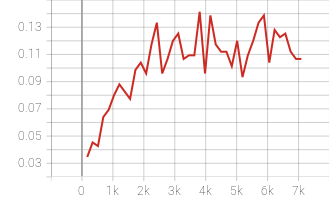
\includegraphics[scale=0.3]{val_rec10.png} & 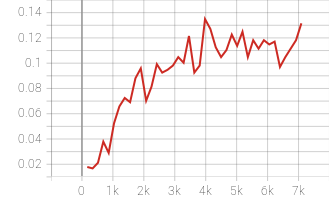
\includegraphics[scale=0.3]{valnarr_rec10.png}\\
  \end{tabular}
  \caption{Validation recall@10 on the retrieval task. The x-axis
    shows the training steps.}
  \label{fig:retrieval}
\end{figure}

\begin{figure}
  \centering
  \begin{tabular}{cc}
    Dialog & Narration \\
    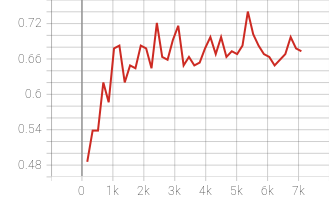
\includegraphics[scale=0.3]{val_acc3.png}  & 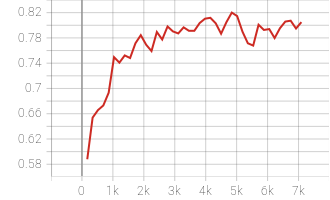
\includegraphics[scale=0.3]{valnarr_acc3.png}\\
  \end{tabular}
  \caption{Validation accuracy on the triplet task. The x-axis shows
    the training steps.}
  \label{fig:triplet}
\end{figure}

\paragraph{Multiple representational similarity analysis}
\Cref{tab:dialog-lm} and \Cref{tab:narration-lm} show the coefficients
of the linear models fit to the dialog and narration pairwise
similarity data respectively. For both datasets the predictors with
the largest effects are {\tt durationdiff} and {\tt glovesim}. The
speaker predictor for the dialog data {\tt samespeaker} is significant
but rather small in size. These results further indicate that the
model learns some aspects of word-level semantics as captured by GloVe
word vectors, and that speaker identity does not appear to be a
substantial impact on utterance embeddings.

\begin{table}
  \centering
  \begin{tabular}{lrrrr}\toprule
            &       Estimate & Std. Error  & $t$-value & $Pr(>|t|)$ \\    \midrule
(Intercept) &  -0.0904846    & 0.0097785   & -9.253  & $<$ 2e-16  \\
glovesim    &  0.2988523     & 0.0057028   & 52.404  & $<$ 2e-16  \\
distance    &  0.0023374     & 0.0013607   & 1.718   & 0.0858     \\  
durationdiff& -0.5893604     & 0.0011985   & -491.729& $<$ 2e-16  \\
sametype    & -0.0007688     & 0.0091374   & -0.084  & 0.9329   \\
samespeaker & -0.0134440     & 0.0018766   & -7.164  & 7.85e-13 \\
sameepisode &  0.0290118     & 0.0015624   & 18.568  & $<$ 2e-16  \\
\bottomrule
  \end{tabular}
  \caption{Association of predictors with model-based pairwise
  similarity scores for single-word utterances in the dialog
  validation data. Indicators are sum-coded ($1$ vs $-1$) while the
  numerical variables are z-scored.}
\label{tab:dialog-lm}
\end{table}

\begin{table}
  \centering
\begin{tabular}{lrrrr}\toprule
             &   Estimate    & Std. Error  & $t$-value & $Pr(>|t|)$\\\midrule
(Intercept)  & -0.3987661    & 0.0013556   & -294.16   & $<$2e-16 \\
glovesim     & 1.0121928     & 0.0009852   & 1027.44   & $<$2e-16 \\
distance     & 0.0078558     & 0.0002042   & 38.48     & $<$2e-16 \\
durationdiff & -0.4665827    & 0.0001662   & -2806.79  & $<$2e-16 \\
sametype     & -0.1566686    & 0.0010152   & -154.33   & $<$2e-16 \\
sameepisode  & 0.0726940     & 0.0007647   & 95.06     & $<$2e-16 \\
\end{tabular}
\caption{Association of predictors with model-based pairwise
  similarity scores for single-word utterances in the narration
  validation data. Indicators are sum-coded ($1$ vs $-1$) while the
  numerical variables are z-scored.}
\label{tab:narration-lm}
\end{table}